\documentclass[11pt,a4paper]{ivoa}
\input tthdefs

\usepackage[utf8]{inputenc}

\title{IVOA Provenance Data Model}

\ivoagroup{DM}

\author{Kristin Riebe}
\author{Florian Rothmaier}
\author{Markus Demleitner}
\author{Adrian Partl}
\author{Jochen Klar}
\author{Mireille Louys}

% \previousversion[????URL????]{????Funny Label????}
\previousversion{This is the first draft}
       

\begin{document}
\begin{abstract}
[TODO]

NOTE: The urls above won't work yet, because this draft is only circulated via the volute-repository for now.
\end{abstract}


\section*{Acknowledgments}

This document has been developed in part with support from the German
Astrophysical Virtual Observatory (BMBF Bewilligungsnummer 05A08VHA).



\section*{Conformance-related definitions}

The words ``MUST'', ``SHALL'', ``SHOULD'', ``MAY'', ``RECOMMENDED'', and
``OPTIONAL'' (in upper or lower case) used in this document are to be
interpreted as described in IETF standard, \citet{std:RFC2119}.

The \emph{Virtual Observatory (VO)} is
general term for a collection of federated resources that can be used
to conduct astronomical research, education, and outreach.
The \href{http://www.ivoa.net}{International
Virtual Observatory Alliance (IVOA)} is a global
collaboration of separately funded projects to develop standards and
infrastructure that enable VO applications.


\section{Introduction}

In this document, we discuss a draft for an IVOA standard data model for describing the
provenance of data. We focus here on observational data, since provenance for
simulated data is already covered by SimDM 
\cite{std:SimDM}. This ProvDM draft is at a very preliminary state and may change at any time.


\subsection{Role within the VO Architecture}

\begin{figure}
\centering

% Get the architecture diagram from the TCG chair
% http://wiki.ivoa.net/twiki/bin/view/IVOA/IvoaTCG
% If they give you a PDF, for now dumb it down to a png by
% convert -antialias -density 72x72 archdiag.pdf archdiag.png
% Oh -- Notes don't need this; you'd have to remove archdiag.png
% from FIGURES in the Makefile, too.

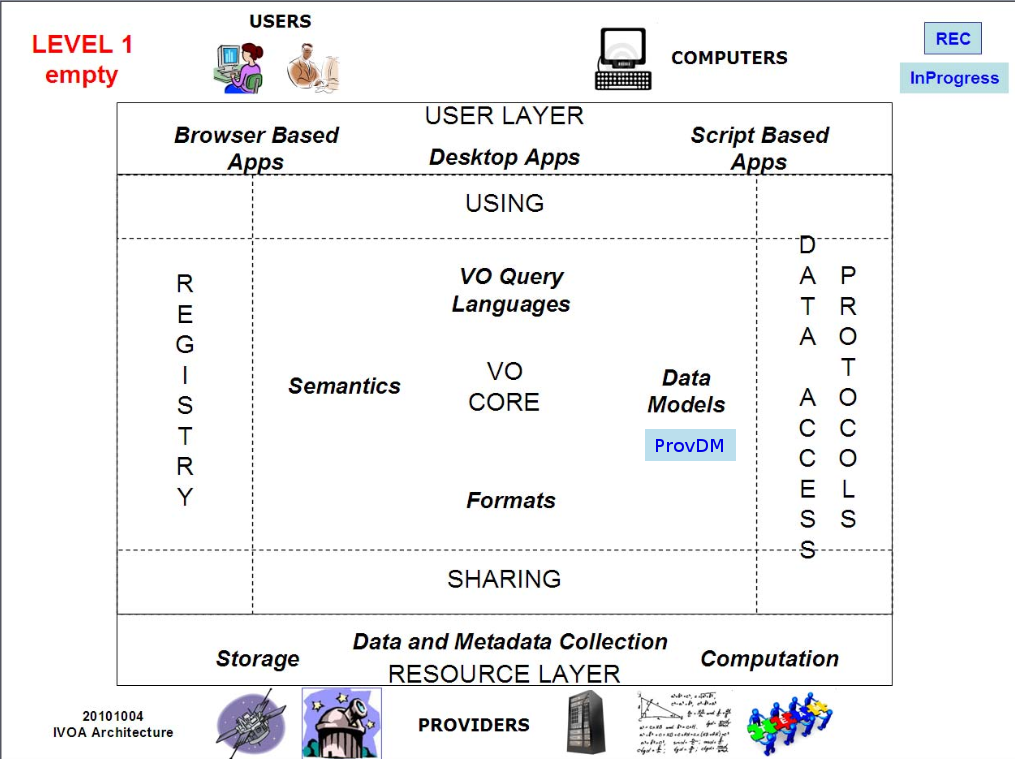
\includegraphics[width=0.9\textwidth]{archdiag.png}
\caption{Architecture diagram for this document}
\label{fig:archdiag}
\end{figure}

Fig.~\ref{fig:archdiag} shows the role this document plays within the
IVOA architecture \citep{note:VOARCH}.


\subsection{Requirements for Provenance and Use Cases}
A provenance data model should provide solutions to the following tasks:
\begin{itemize}
\item   \textbf{A: Tracking the production history}\\
		Find out which steps were taken to produce this piece of data/image and which methods/tools/software was involved. 
		Track the history back to the raw data files/raw images.

		Examples: 
		\begin{itemize}
			\item Is the image from catalogue xxx already calibrated?
What about dark field subtraction? Were foreground stars removed? Which technique
was used?  
			
			\item Is the background noise of atmospheric muons still present in my neutrino data sample?  
		\end{itemize}

		We don't go so far as to consider easy reproducability as a use case -- this would be too ambitious. But at least the 
		major steps undertaken to create a piece of data should be recoverable.

	  

	\item   \textbf{B: Attribution and further information}\\
		Find the people involved in the production, the people/organizations/institutes that need to be cited or can be asked for more information

		Examples: 
		\begin{itemize}
			\item I want to use an image for my own work - who was involved in
creating it? Whom do I need to cite or who can I contact to get this information?  
			\item I have a question about column xxx in the data
table. Who can I ask about that?  
		\end{itemize}
	  

	\item   \textbf{C: Aid in debugging}\\
		Find possible error sources.

		Examples: 
		\begin{itemize}
			\item I found something strange in an image. Where does
the image come from? Which instrument was used, with which characteristics
etc.? Was there anything strange noted when the image was taken?  
			\item Which pipeline version was used -- the old one
with a known bug for treating bright objects or a newer version?  
			\item This light curve doesn't look quite right. How was
the photometry determined for each data point?  
		\end{itemize}

	  

	\item   \textbf{D: Quality assessment}\\
		Judge the quality of an observation, production step or data set.
		
		Examples: 
		\begin{itemize}
			\item Since wrong calibration images may increase the
number of artifacts on an image rather than removing them, the knowledge about
the calibration image set will help to assess the quality of the calibrated
image.  
		\end{itemize}
	  

	\item   \textbf{E: Search in structured provenance metadata}\\
		Find all images produced by a certain processing step and similar tasks.
		
		Examples: 
		\begin{itemize}
			\item Give me more images that were produced using the
same pipeline.  
			\item Give me an overview on all images reduced with the same calibration data set.  
			\item Are there any more images attributed to this observer?  
			\item Which images of the crab nebula are of good quality and were produced within the last 10 years by someone not from ESO or NASA?  
		\end{itemize}

		This task is probably the most challenging. It also includes tracking the history of data items as in A, but we still have listed A separately, since we may decide that we can't keep this one, but we definitely want A.
	  
\end{itemize}


\section{Previous efforts on provenance modelling}
\subsection{Provenance in the IVOA}

Provenance was already discussed since the early days of the IVOA, but previous efforts from the IVOA community unfortunately are mostly not well documented or we were not able to find them. 
There exists a vocabulary list by Arnold Rots, we got a provenance diagram from a talk by Francois Bonnarell, and there exist workflows to track provenance for specific projects (e.g. CTA), but this is all very specific and too detailed for a general provenance model. We therefore went a step back to start with a more abstract core model as discussed in this document.

\emph{TODO: give more specific references, check other data models and where they touch provenance}


\subsection{Open Provenance Model (OPM) and W3C PROV-DM}

Other communities have put considerable efforts into establishing a provenance model.
The Provenance Challenge series (2006 - 2010) was a community effort to achieve inter-operability between different representations of provenance in scientific workflows. It resulted in the Open Provenance Model (\cite{moreau2010}), and some members of that challenge continued their work by joining the W3C Provenance Working Group. The W3C Provenance Data Model was released as Recommendation in 2013. The cores of OPM and W3C are in principle the same, therefore we focus here on describing the basic concepts of the W3C Provenance Data Model (PROV-DM, see \cite{std:W3CProvDM}).


OPM was designed to be applicable to anything, scientific data as well as cars or immaterial things like decisions. With W3C, this becomes more focused on the web. Nevertheless, the core concepts are still fairly general and should be useful for astronomical data sets as well, though we could aim at making it more specific and less abstract for our purposes. 

The elements of a provenance model can be expressed as a directed graph to capture the causal dependencies. In W3C, there are three core components, i.e. nodes of the graph:
(see Section 1+2 and Fig. 1 in \cite{std:W3CProvDM} for the detailed specification, which we reproduce here only partially):

\begin{itemize}
\item Entity: a thing, at a certain state (car, paper, data set, idea)
\item Activity: an action/process or series of actions, occurs over a period of time, performed on or caused by entities, usually results in new entities
\item Agent: executes/controls an activity
\end{itemize}

There are also different possible relations between these components. Those important for astronomical data are:
\begin{itemize}
\item Generation: a new entitiy is generated by an activity (output\_data wasGeneratedFrom activity)
\item Usage: an entity is used by an activity (activity used input\_data)
\item Association: agents have responsibility for an activity (agent wasAssociatedWith activity)
\end{itemize}

There is one more relation that could be interesting for us:
\begin{itemize}
\item Attribution: an entitiy can be attributed to an agent (entity wasAttributedTo agent)
\end{itemize}
The attributed-to-agent may be different from the agent that is associated with the activity that created an entity.

Figure \ref{fig:w3cclasses} summarizes the (core) classes and relations of the W3C provenance model that are interesting for us.

\begin{figure}
\centering
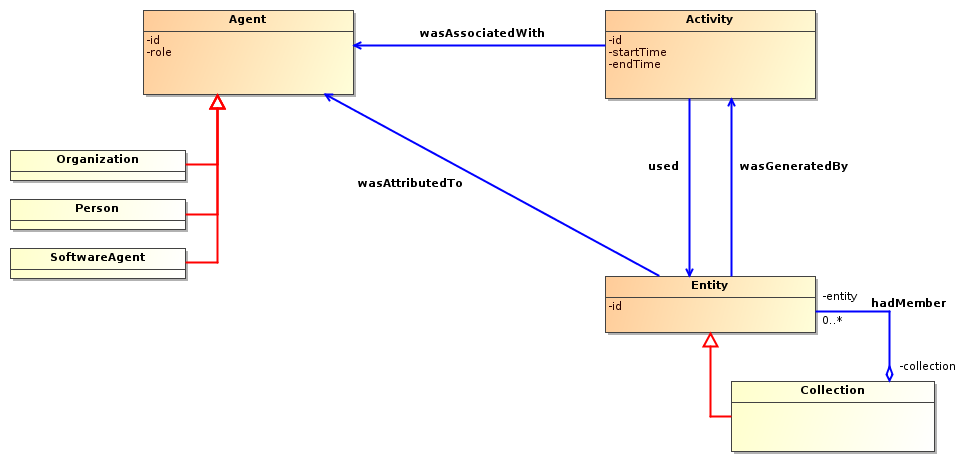
\includegraphics[width=0.8\textwidth]{ProvDM-W3C-classdiagram.png}
\caption{The main classes and relations of the W3C Prov-DM, that could be useful for the VO.}
\label{fig:w3cclasses}
\end{figure}


The W3C PROV-DM further specifies a Derivation relation, which directly links a derived entity to its predecessor. This was introduced to make the link between entities more explicite. If activity a used entities e1 and e2 as input and produced e3 as output, then it is not clear, if e3 is a derivative (or, in W3C terms, "wasDerivedFrom") e1 or e2 or both or neither. e1 and e2 could have been only parameter files for an observation.  

However, for the IVOA provenance model we are fairly sure that this is not needed. Instead, at the moment we favour adding a \emph{role} to each dataItem or entity, which can explain in more detail in which way the entity was used.

We will discuss later an approach using the additional Method-class as prototype or template for each activity.
The types of input/output data and their roles are described using additional classes for the method, so that any kind of relation between input/output data can be covered.

One of the important details here is that e.g. many data sets used by one activity may have different roles for that process (one file is a parameter file, another one is the raw image, and the third one is the dark field that should be subtracted). Since these roles are very important for an activity, they have to be included in the provenance model.

These roles don't have to be unique (see \cite{moreau2010}, after Definition 10), many data sets may have the same role for a process (e.g. raw image input).
The IVOA community should specify and describe the possible roles for each method (which is the template for the activity), in order to facilitate interoperability. A vocabulary list or thesaurus could be useful here.

OPM also suggests to allow hierarchical descriptions, i.e. allow to include different ways of getting from data set a to data set b, with different levels of detail. 
This needs to be discussed further. 
(After talk at InterOp-Madrid, May 2014, some people said that this would be important for them!)

W3C describes a collection as an aggregation of entities. This is a useful concept to adapt here, since it allows to treat many data (e.g. the RAVE survey) as one entity.

It is possible to extend the core model of the W3C provenance model by using the PROV-DM Extensibility points (section 6 in \cite{std:W3CProvDM}). This allows to specify additional roles and types to each entity, agent or relation using the attributes \texttt{prov:type} and \texttt{prov:role}.
By specifying the allowed values for the IVOA model, we can adjust the model to our needs while still being compliant to W3C.





\emph{TODO: more details about W3C; explain reasons, why the other relations (e.g. Communication) are not needed. Should we include specific agent-relations like attribution, delegation?}



\section{A Provenance Data Model}
We describe here the core concepts for modelling provenance. The resulting model could then be reused as a kind of pattern everywhere where provenance is needed in the VO. [TODO: How exactly may be described here as well or even in the other data models.] 


Currently, we are still debating which way to go: a model using prototypes similar to \cite{std:SimDM} or rather a variant of the W3C-model.
We present them here along with some of their advantages/diadvantages.

\subsection{A model using prototypes}
This model is inspired by \cite{std:SimDM}, a data model for simulation data published in May 2013. Especially we copied the central classes: Protocol and Experiment.  A Protocol is the plan or method
which describes how to do something whereas Experiment is the actual execution of
this plan. Defining such protocols allows them to be reused, which is very useful when performing series of experiments of the same type, as is typically done in astronomy. For our provenance mdoel, we use the more generic term
\texttt{Activity} instead of Experiment, as it us used by the W3C Provenance Data Model (\cite{std:W3CProvDM}). Instead of \texttt{Protocol}, we use the term \texttt{Method}, 
for not confusing it with e.g. IVOA protocols.

The class diagram generated with MagicDraw Community Edition is given in the figure\ref{fig:classes-prototypes}; the details are described in the next sections.

\begin{figure}
\centering
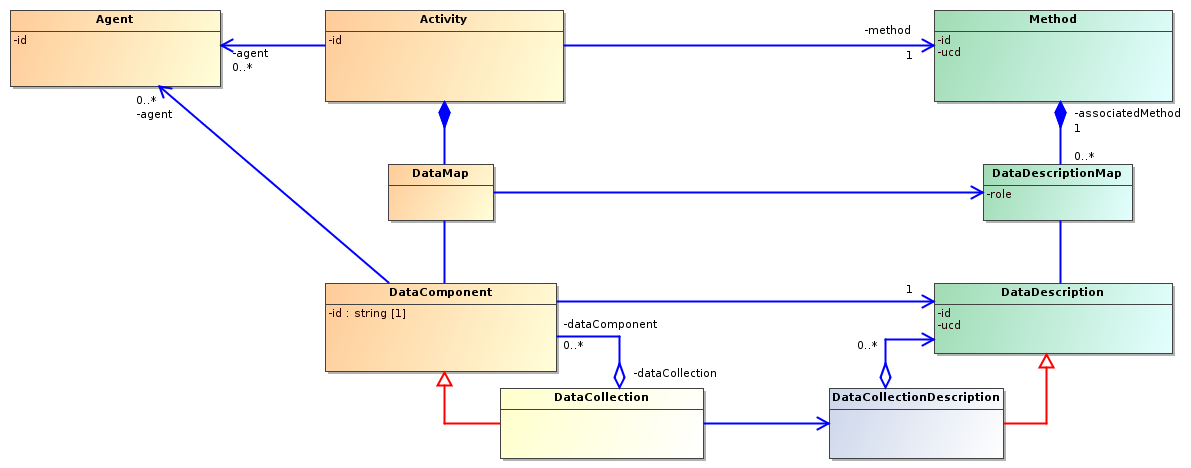
\includegraphics[width=0.8\textwidth]{ProvDM-classdiagram-prototypes.png}
\caption{The (current) Provenance Data Model
class diagram. It will certainly change again, so use it with care. In this version, we stripped it now from nearly all derived classes, so we can concentrate on the core elements. The green and blue boxes belong to 'prototype' classes.}
\label{fig:w3cclasses}
\end{figure}

\subsubsection{Activity and method}
Activity corresponds to Experiment and Method to Protocol from \cite{std:SimDM}.

Examples for astronomical activities are observations and processing steps like
flat-fielding, correcting bias, astrometric calibration etc. The type or method
underlying an activity is specified by the corresponding \emph{Method} class.
This could be, for instance, the name of the code used to perform an activity or a more general description. An activity is a concrete case of using such a method, thus it has to refer to a corresponding method. 


There MUST be exactly one method per activity. If steps from a pipeline shall be 
grouped together, one needs to create a proper method for describing all 
the steps at once. This method can then be refered by the pipeline-activity. 

\subsubsection{Data and DataDescription}
We define a general \texttt{Data} class (actually: DataComponent, see next section), 
which can represent either an individual data item or a collection of data. The W3C equivalent to this class is called \texttt{Entity}, but we use \texttt{Data} instead, since we do not aim to model cars and abstract ideas here, but more concretely astronomical data of any kind. 

Following the scheme that each \texttt{activity} is described
by the more general \texttt{method}, we associate each input or
output data set with a corresponding description of the data type. Each method
usually makes assumptions on the structure of input data (FITS file, data
table, binary file of a certain structure ...) and produces a certain form of
output data, which should be described in the general \texttt{DataDescription}
class, so that it can be reused for multiple instances of this class.


There has been some dispute (before and at the InterOp in Madrid, May 2014) about the different roles of input and output data. Since the results of one activity can be input data for
another activity, the structure of input and output data is necessarily the same.
The link from an \texttt{Activity} to the corresponding \texttt{Data}
object could tell then if the piece of data is used as input or output, see Figure~\ref{fig:activities} in section \ref{sec:links_between_data}.
% (see figure at <span class="xref">links_between_data</span>).

However, input data can take different roles in an activity (auxiliary data like a parameter file, two images, with one that needs to be subtracted from the other) and it must be made explicit which data component that is used by or generated from an activity fulfills which role. In W3C, this is partially solved by adding a derivation relation between the entities (data). Here, we add a mapping-class between activity and data as well as between method and dataDescription. The mapping-class at the description side, i.e. between the Method and its DataComponentDescriptions, contains additionally a role for each relation, e.g. parameter, dark frame, raw image, etc.  If a dataComponent is used as input to an activity or if it results from it, will become clear with these roles.

\emph{Note: Suggestion by Jochen: What about defining a Role-class for methods? This way each method should define the roles that are allowed for the method (probably taken from a specified list of vocabularies), enhancing inter-operability.}

Without the mapping tables, the relation between activity/method and data/datadescription would be an aggregation relation, or in other words: an association with the aggregationKind "shared". That would be required to ensure that all DataComponents linked to an activity (either as input or output) will survive if the activity is destroyed, since they are almost always shared with other activities. 

By using the mapping tables we make the role of a dataComponent in an activity more explicit and thus can replace the aggregation by a composition relation to the activity/method and simple associations to the individual data components and their descriptions. 


\subsubsection{Data Collections - Composite pattern}

There are two major data classes: 

\begin{itemize} 
\item data collections \\e.g. RAVE-DR4 with its databases and database tables, SDSS DR9 with 
all its tables and files, all files from one observing slot\\

\item individual data components\\
e.g. a file, table in a database, parameter value, an image, a fits-file containing a table and image

\end{itemize}


Data can only be grouped to a data collection, if they have the same origin (i.e. they were
produced by the same activity, i.e. they have the same provenance).
We would leave it to the person/tool recording provenance to decide, how detailed a data set will be  
separated into individual items. It is also possible to just record provenance for e.g. RAVE DR4 as a 
whole, without listing everything that belongs to DR4. The level of detail could then be specified via 
the DataDescription.



For our data model, it would be desirable to be able to treat data collections and individual data items in
the same way, with the same interface. This demand led us to the 
\textbf{Composite design pattern}:


We introduce an abstract class called \texttt{DataComponent}, which 
includes the basic properties and functionality for both, data items like files or 
parameter values or a complete data set. Such common properties are e.g. the link 
to the activity which created the data/dataCollection, a creation date/time and a link to a
storage-object (which is not further specified in this data model).

Each DataComponent can either be a single item (like a file, database table or a parameter) 
or a DataSet. A DataCollection contains additionally a (non-empty) list of child-DataComponents, 
which could again contain a list of 
further children etc. This way, one could represent complete data trees, if necessary.

Each DataComponent also has a link to its parent, which would be 
emtpy (or point to itself) for the root-DataComponent.

We hope that such a representation would make it easier for clients to handle data 
objects, since they don't have to make the distinction between data items and data 
collections. 


\subsubsection{Agent}
In SimDM, someone performing a certain experiment is called \texttt{Contact}, 
the W3C provenance data model suggests the term \texttt{Agent}, so we adopted it here.
We want to describe someone who is responsible for an activity, e.g. who pressed a button, 
ran a script or performed the observation. The agent could be a single person 
(specified by name), a group of persons (e.g. MUSE WISE Team), project/organization (RAVE) or an institute. 
For each of them a name should be specified.

It is desired to have an agent given for each activity, but it
is not enforced (hence 0..*).  It would also increase the value of the given
information if the (current) affiliation of the agent and a project leader/group
leader were specified in order to maximize the chance of finding someone later
on. The agent should not only be used for getting contact information, but also 
to fulfill our "Attribution" requirement, so that proper credit goes to the right 
people/projects. To this end, it could also make sense to add a relation between a DataComponent and Agent, similar to W3C's wasAttributedTo-relation.


\emph{TODO: Specify pre-defined contact or agent roles to choose from, in order to maximize interoperability (see SimDM: owner, creator, publisher, contributer; any more?)}


\subsubsection{Storage}
The modelling of storage is not included in this model. 
It would be useful to be able to make a reference from the DataComponent to a storage
object that contains the link to where the data is stored. But we haven't fixed the 
details here.


\subsubsection{Links Between Data}\label{sec:links_between_data}
It would be convenient if each data object or even each file (\texttt{Storage object})
gets a unique \texttt{dataId} that can be referenced. If several copies have been
made out of a data set and one of them is corrupted, it would even be useful to know
exactly which copy was used by a given activity. 

\emph{Maybe DataLink can help here? Or DOIs?}

We need to be able to refer from an activity to the ResultData of another
activity. A possible data flow is shown in the figure below:

\begin{figure}
\centering
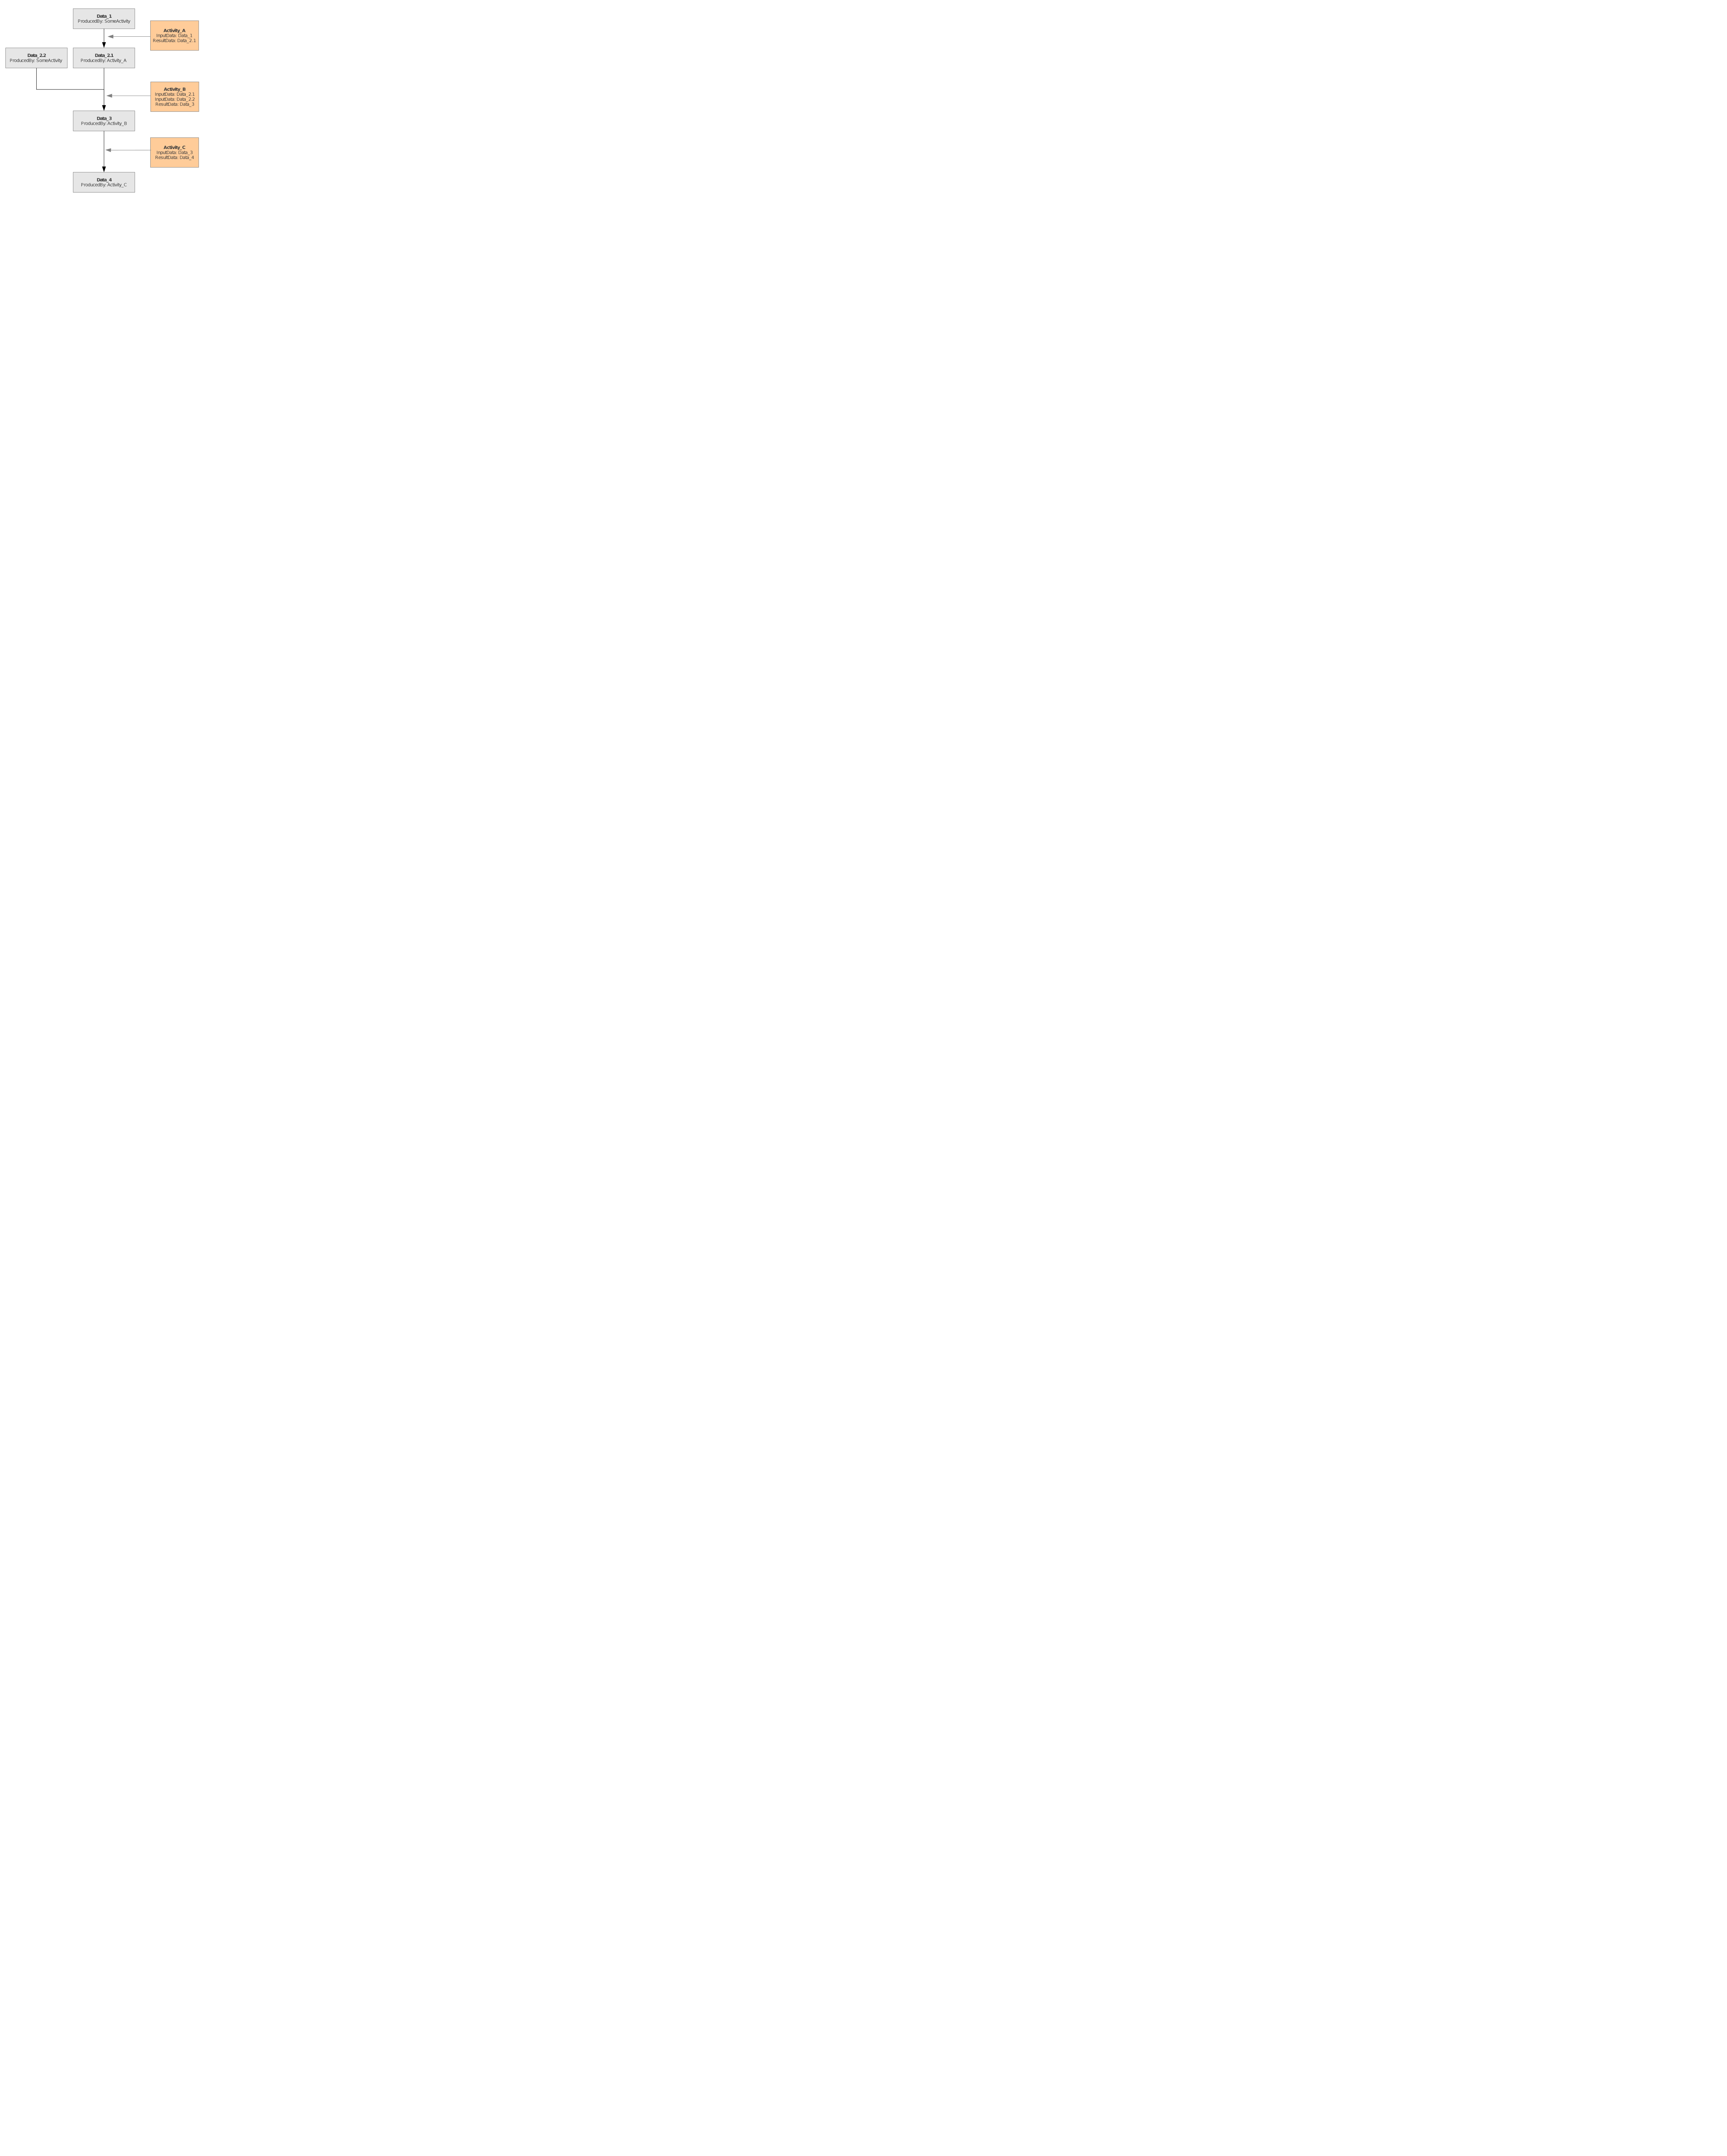
\includegraphics[width=0.8\textwidth]{ProvDM-activities.png}
\caption{The black arrows indicate the
data flow, gray lines just show which activity would be attached to the step. It
is defined by the role in the corresponding Activity whether data is used as input
or output.}
\label{fig:activities}
\end{figure}



\subsubsection{Calibration data}
The calibration data set consists of images that can be used to calibrate the
raw data. It is not necessary to mention them explicitly in the model, they are just another dataSet that is used by activities with a calibration-method.


\subsubsection{Ambient Conditions}

Ambient conditions are environmental properties, which are special in a way: 
they represent the part of an activity, usually an observation, which cannot be 
(fully) controlled by an
observer, in contrast to other data that can be fully reproduced.
Nevertheless we decided that they can be fully described by our 
data class already and don't need a separate class in our data model. 

Our model can then also take into account that a certain observation
method requires special ambient conditions, already defined via the method
(e.g. radio observations rely on different ambient conditions than observations
of gamma rays), just following our data - data description scheme.


Ambient conditions are recorded for a certain time (executionDate) and are
usually only valid for a certain time interval. This time interval should be recorded
with a validity-attribute for DataComponents.


\emph{We wondered if ambient conditions could also play a role for some
processing steps or any other activity besides observations? Is there any
additional step performed in which room temperature etc. may play a role and thus
should be recorded? The only example that came to our minds was the storage of
photographic plates, where the humidity and temperature variations can affect the
quality of the photographic plates.}



\subsubsection{Instrument Characteristics}
In contrast to ambient conditions, instrument characteristics do (usually) not
change from one observation to the other, so they are static, strictly related to
the instrument. 
All the characteristics could be described either as key-value pairs directly with the 
observation or just as data, using the DataComponent class. One would then 
link the instrument characteristics as a type of input data set to a certain 
observation activity. Thus we don't need a separate Instrument or Device class.



One should also keep in mind that some instrument related parameters can change within time,
e.g. the CCD temperature. The instruments can also change within time because of aging.


\subsubsection{Quality}
We could simply define additional attributes for each \texttt{Activity}
or \texttt{Data} object, i.e. zero, one, or more properties in the form of
key-value pairs. We could use a \texttt{Quality} namespace to mark a keyword
as quality-related:
\begin{itemize}
	\item quality.comment: [some text]
	\item quality.seeing: [some value]
\end{itemize}
The values could range from a float number to free text.

\subsubsection{Discussion}
This model was established with having a database implementation in mind. However, we'll look again at W3C in the next section, which may offer simpler possibilities to store provenance with the dataComponents themselves, e.g. as an additional structure in fits-headers.


A model using prototypes has the advantage of normalisation: methods could be described once and for all at some place (this \emph{some place} is actually the crucial point here!) and then be reused when describing the actual provenance of certain dataComponents and activities.
However, building such a look-up place for all the possible methods and dataDescriptions is a quite challenging task -- it will probably never be complete. There's also the issue of persistent identifiers/broken links to consider.
Normalisation is useful for closed systems, e.g. for describing the provenance for data produced by a certain pipeline (e.g. MuseWise system) or with workflow tools or when a task needs to be repeated many times. However, the VO is quite the contrary of a closed system and we need to keep an eye on what is actually achievable.


\subsection{A simpler model based on W3C}


When trying to write down a simple serialisation of e.g. the provenance for a stacked image with the protoype-model, it soon becomes quite cumbersome to define everything twice: first the descriptions, then the instances. This basically doubles the number of entries to describe provenance (unless there is already some place with all the descriptions to which we can refer).


Thus, we consider the W3C-model again, and adjust it by replacing the used- and wasGeneratedFrom-relations by a mapping class between activity and entity in the following class diagram:

\begin{figure}
\centering
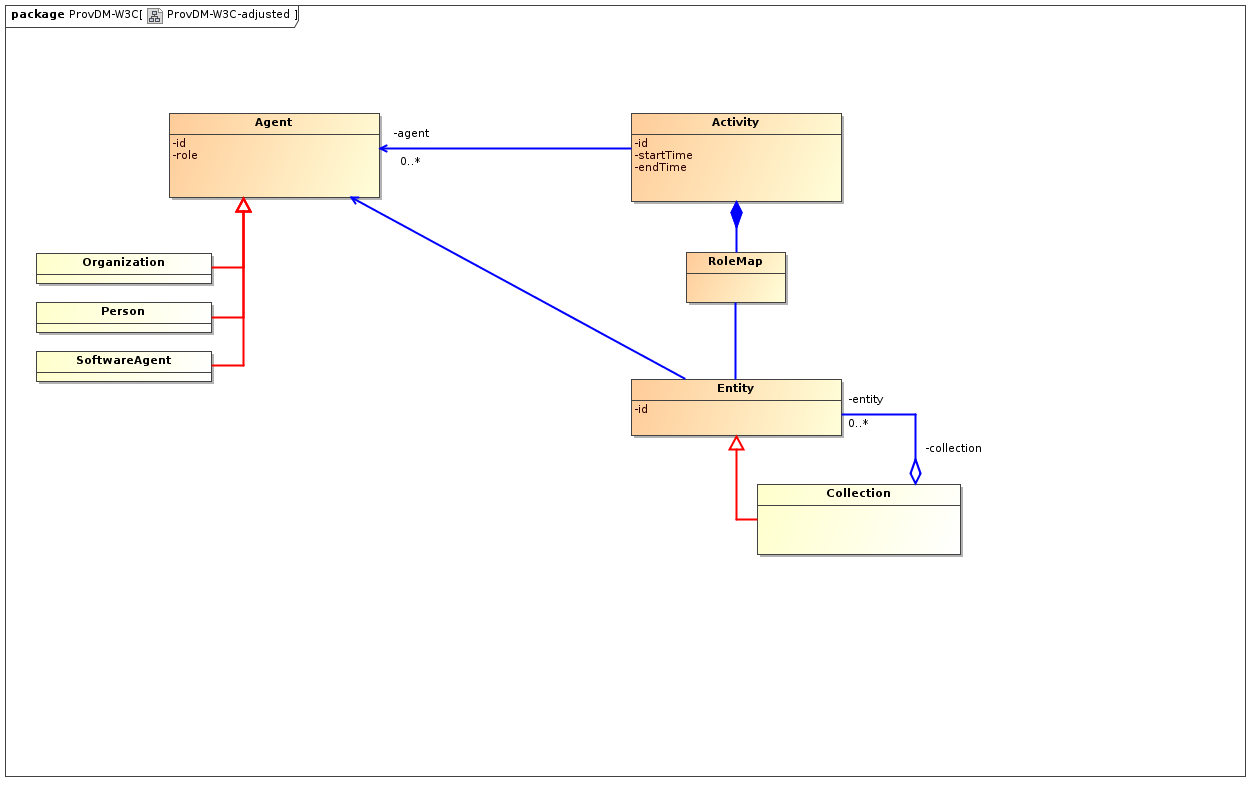
\includegraphics[width=0.8\textwidth]{ProvDM-W3C-adjusted.png}
\caption{An adjusted W3C model for provenance of astronomical data.}
\label{fig:classes-w3c-adjusted}
\end{figure}


The different methods and data types are here hidden in pre-defined vocabulary lists. 
An example for writing down the provenance for a stacked image in W3C and with the protoype-model is given in the accompanying files 
\texttt{prov-example-incl-prototypes.txt} and 
\texttt{prov-example-w3c.txt} at \href{https://code.google.com/p/volute/source/browse/trunk/projects/dm/provenance/description/}{volute}.




\subsubsection{Discussion}

Expressing provenance for a stacked image with this smaller set of classes may be simpler, but on the other hand constructing a database schema becomes much harder. 

The question is: could we just derive a simple exchange format from the prototype-model? Should we be instance-driven here? Which model would be more useful?




\appendix
\section{Changes from Previous Versions}
%\subsection{Changes from previous version}
%Transformed from ivoadoc to tex-version.
% No previous versions yet.  
% these would be subsections "Changes from v. WD-..."
% Use itemize environments.


\bibliography{ivoatex/ivoabib,prov-refs}


\end{document}
